\documentclass[../../main.tex]{subfiles}

 \lhead{Project Management}
 
\begin{document}

\section{Project Management}
	Upon starting the project, a simply Gantt chart was constructed to lay out the task that needed to be complete and the approximate time scale that should be allocated to each one. Very little of the project objectives changed from the initial planning other than one task which was producing low frequency accurate synthetic \ac{RIR}'s which would have taken a significant amount of time. As they would have taken a significant amount of time to produce and the project could be completed without.

	Two weeks into the project it was decided that the Gantt chart was not an appropriate method for project planning. This is because some tasks (such as producing synthetic \ac{RIR}'s) relied solely on the completion of the preliminary tasks and once it was discovered that room modelling would take a lot longer than originally thought due to inexperience with such as task, the Gantt chant would have had to be redesigned which would have taken even more tie today. Instead, a series of check lists were used to keep track of which tasks needed completing. These tasks were written on post-it notes and used in a large Kanban bored situated on the authors bedroom wall, seen in figure~\ref{kanban}

	Figure~\ref{gantt} in \nameref{appendixE} shows the initial Gantt chart with a red line indicating at what point it was abandoned for a more appropriate planing method. Along with this, weekly emails were sent to the projects supervisor with an update regarding the progress of the project and any problems that were faces, as well as regular meetings with both the projects supervisor and a larger group of students with audio related projects.


	\begin{center}
	\begin{figure}[H]
		\vspace{50mm}\centerline{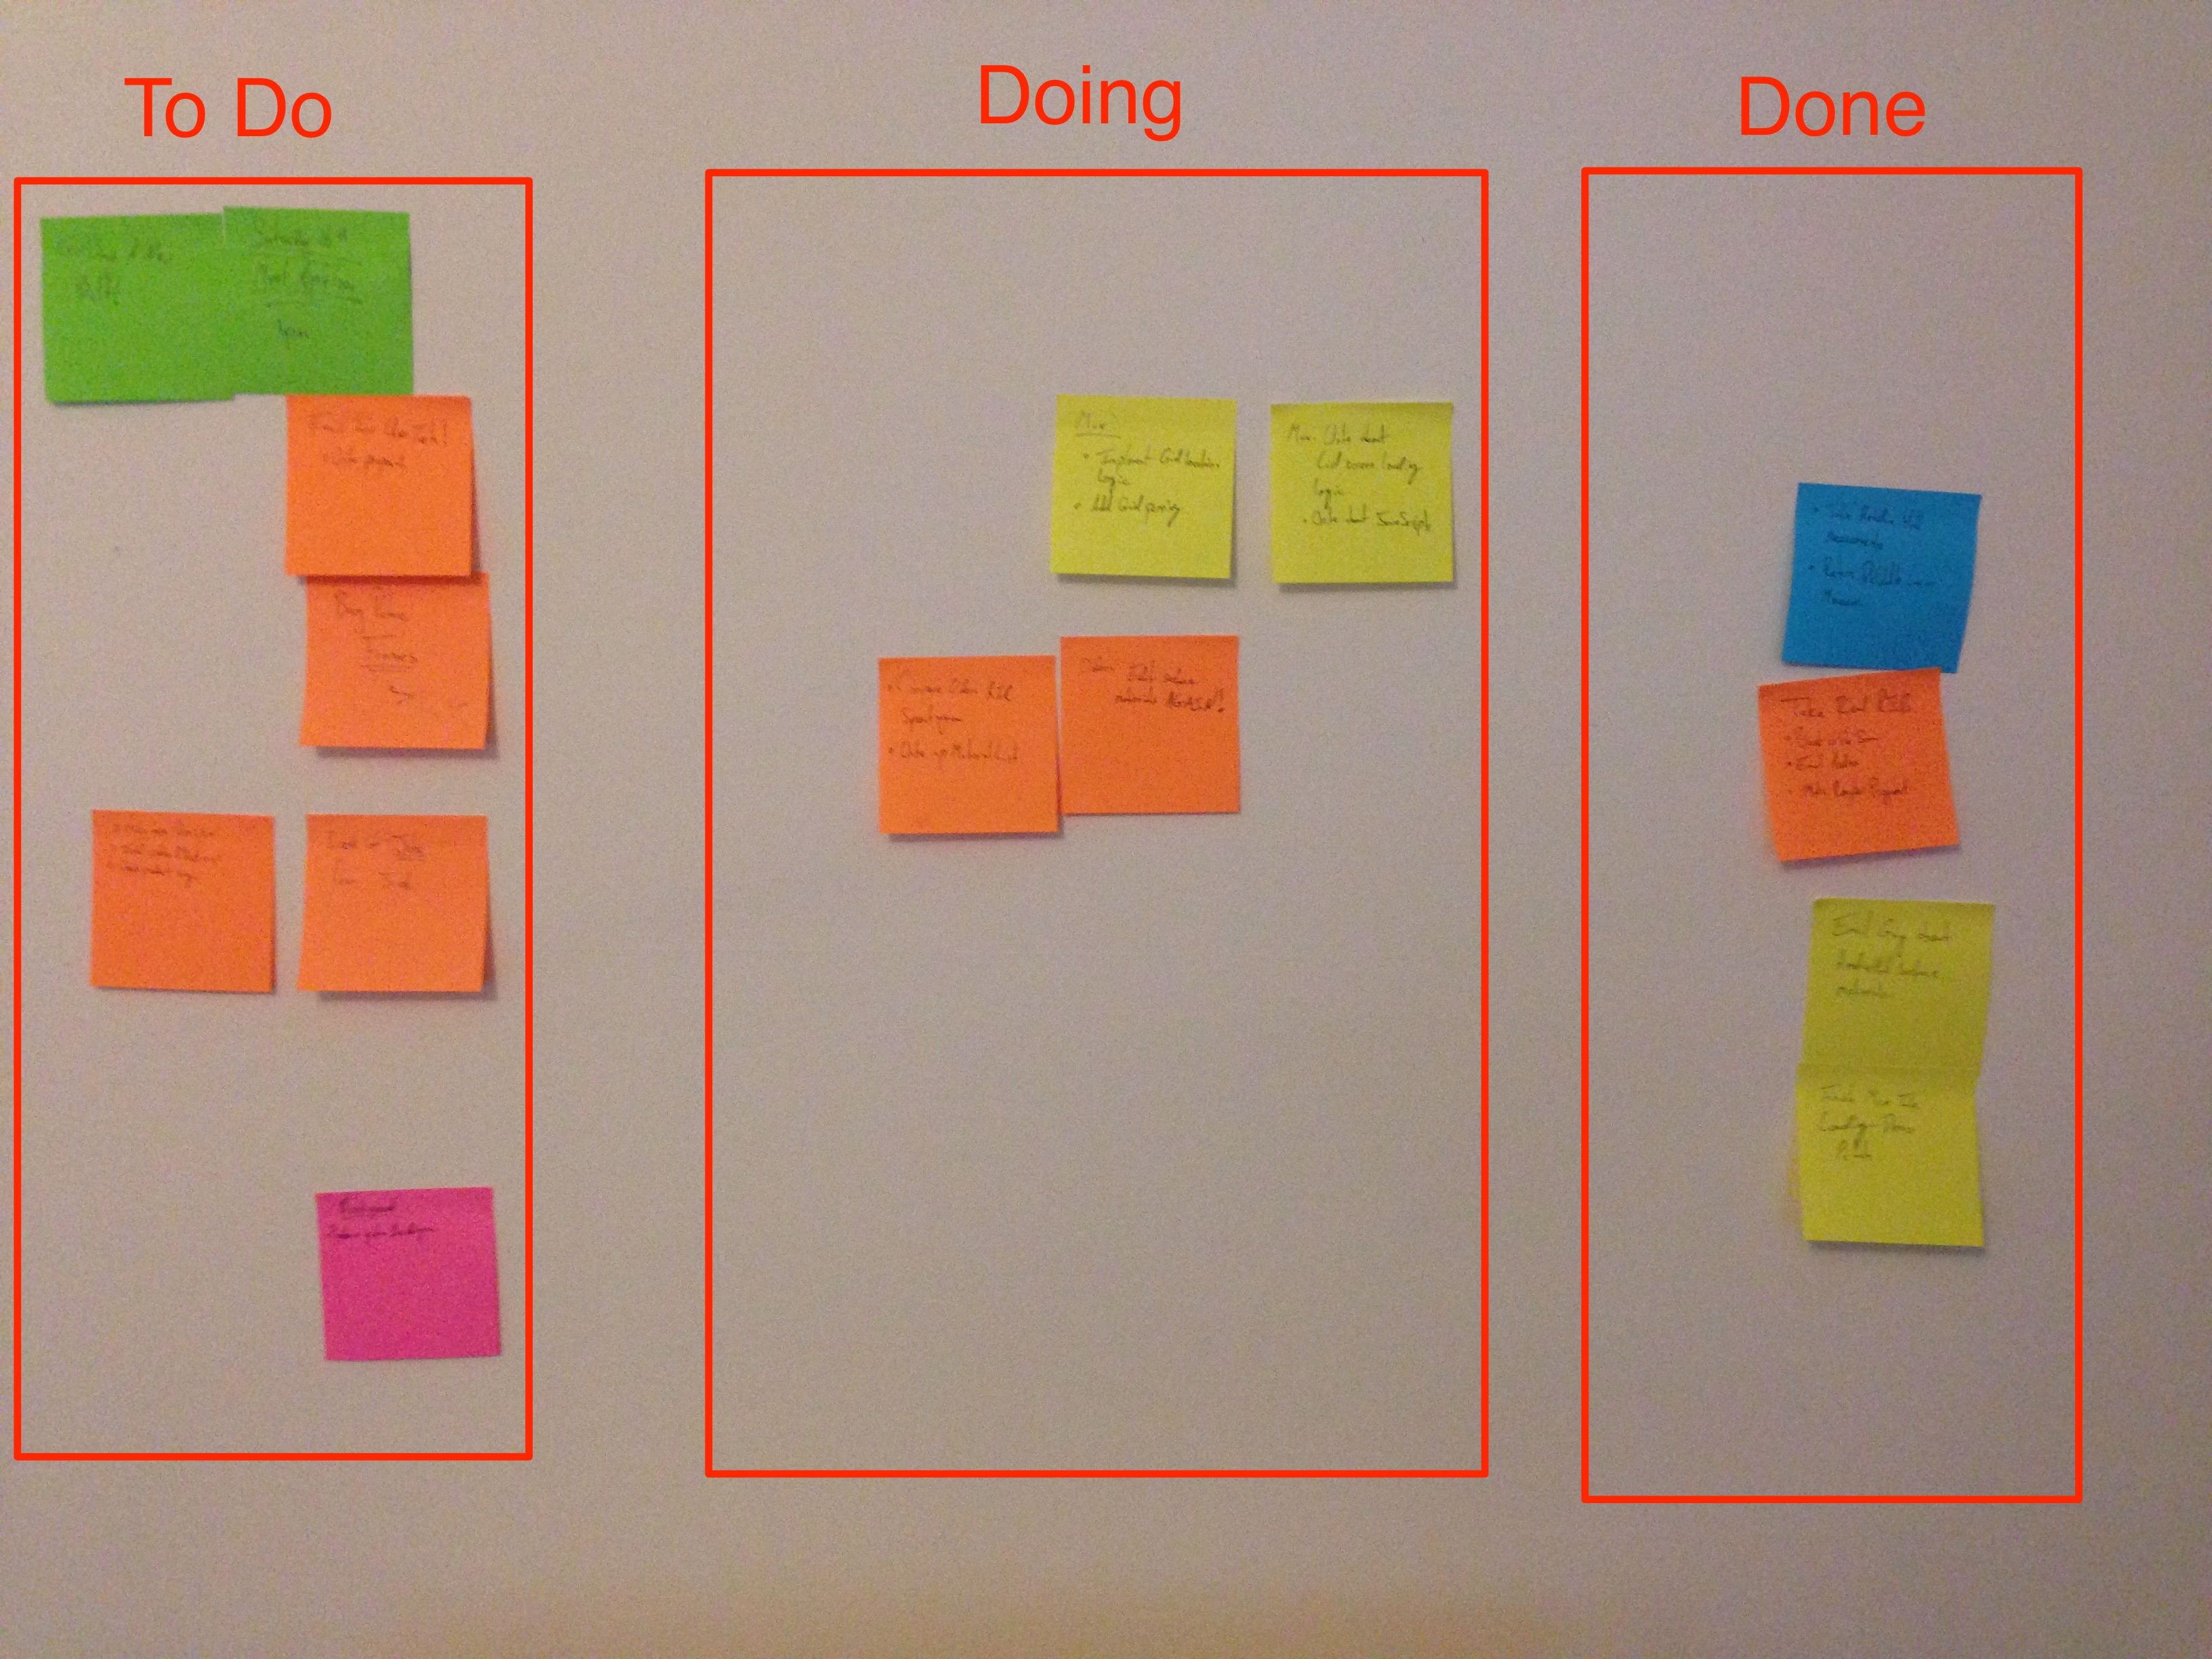
\includegraphics[scale = 0.15]{Sections/ProjectManagement/images/kanban_edit.jpg}}
		\caption{Initial Gantt chart showing the approximate time allocated to each of the tasks required to complete the project. The red line shows the time at which the Gantt chart was abandoned for a more appropriate planning method}
		\label{kanban}
	\end{figure}
	\end{center}


\end{document}